%--------------------------------------------------------------------
% Эта преамбула с комментариями для написания лабораторных работ по
% физике. В еe основе информация из книги С. М. Львовского "Набор и
% верстка в пакете Latex", а также материалы по курсу "Документы и
% презентации в Latex" от ВШЭ https://www.coursera.org/learn/latex. Ну
% и мой опыт (1 год и 16 лабораторных работ + 2 Вопроса по выбору)
% Автор - Баринов Леонид
% Дата - 06.08.2019
%--------------------------------------------------------------------
%--------------------------------------------------------------------
% Для начала необходимо определиться с типом документа. Оптимальный
% (на мой взгляд) вариант - article. Также существуют типы book,
% report, proc и другие. Также в необязательном аргументе можно
% указать тип страницы и размер шрифта. Стандарт по умолчанию - А4 и
% 12 (иногда 10) шрифт. Необязательный аргумент шрифта может принимать
% только 3 параметра - 10, 11, 12 (pt).

\documentclass[a4paper, 12pt]{article}

%--------------------------------------------------------------------
% Чтобы использовать другие размеры шрифта используется пакет
% extsizes. Он позволяет указывать в \documentclass такие размеры - 8,
% 9, 10, 11, 12, 14, 17, 20 (pt). При указании других размеров могут
% возникать различные проблемы.

\usepackage{extsizes}

%--------------------------------------------------------------------
% Необходимо определиться с кодировкой документа. Идеального варианта
% для русского языка не существует - каждый чем-то немного плох. Для
% особо интересующихся - Приложение И в 5 издании книги Львовского. Я
% воспользовался вариантом, предлагаемым на курсе по Latex от ВШЭ.

\usepackage[T2A]{fontenc}
\usepackage[utf8]{inputenc}

%--------------------------------------------------------------------
% Для соблюдения типографских традиций (оказывается такие существуют)
% различных стран создан пакет babel. Самое заметное его действие -
% latex научиться переносить слова того языка, который вы укажите.
% Можно указать несколько языков через запятую. Основной язык
% документа указывается последним.

\usepackage[english,russian]{babel}

%--------------------------------------------------------------------
% Перейдем к заданию полей документа. Есть несколько способов, но
% самый простой из них - это воспользоваться пакетом geometry, который
% позволяет определить все поля документа (начиная с краев листа, что
% важно, так как некоторые другие способы позволяют это сделать только
% косвенно)

\usepackage{geometry}
\geometry{top=25mm}
\geometry{bottom=35mm}
\geometry{left=35mm}
\geometry{right=20mm}

%--------------------------------------------------------------------
% От полей логично перейти к колонтитулам. Тут нам поможет пакет
% fancyhdr. Для него существует 6 колонтитулов - верхний, левый;
% верхний, по центру; верхний, правый и такие же нижние. По умолчанию
% номер страницы находится снизу по центру, а также существует
% линейка, очерчивающие верхний колонтитул. Мне показалось интересным
% сделать колонтитулы схожие с колонтитулами в лабнике. 

\usepackage{fancyhdr}
\pagestyle{fancy}
\renewcommand{\sectionmark}[1]{\markboth{#1}{}} 
% \renewcommand{\headrulewidth}{0mm} % Если необходимо убрать линейку,
% или изменить ее длину
% \lfoot{} % Нижний левый
% \rfoot{} % Нижний правый
% \rhead{} % Верхний правый
% \chead{} % Верхний в центре
\lhead{\thepage} % Номер страницы в левом верхнем углу
\cfoot{} % Оставить нижний колонтитул без цифры

%--------------------------------------------------------------------
% Самое время научиться работать с формулами. А точнее добавить пакеты
% от Американского математического общества, которые позволять
% пользоваться большим количеством математических символов.

\usepackage{amsmath,amsfonts,amssymb,amsthm,mathtools}

%--------------------------------------------------------------------
% Также очень хочется пользоваться русскими буквами в формулах, для
% этого подключаем пакет mathtext, который добавляет окружение
% \text{}. Внутри него можно писать русские буквы в математическом
% режиме.

\usepackage{mathtext}

%--------------------------------------------------------------------
% Большим преимуществом вашего pdf документа будет возможность поиска
% в нем по словам или буквами. (Например, в Ивановнике это
% невозможно)

\usepackage{cmap}

%--------------------------------------------------------------------
% Куда же в физике без картинок и графиков? Давайте исправим
% эту недоработку

\usepackage{graphicx}
\graphicspath{images/} % Необходимо, если рисунки
% находятся в другой папке

%--------------------------------------------------------------------
% graphicx не позволяет вставлять обтекаемые рисунки, но на
% практике они очень нужны. Для этого существует пакет wrapfig

\usepackage{wrapfig}

%--------------------------------------------------------------------
% latex вставляет рисунки по определенному алгоритму. Его,
% конечно, можно менять, но это не настолько просто. Как
% правило, хочется, чтобы картинка располагалась там, где мы это
% указали в коде. Для этого существует несколько пакетов, один из
% них floatrow. Он позволяет для окружения figure указывать
% необязательный аргумент - H (именно большое h), что на latex'овском
% языке означает: вставить картинку здесь и только здесь. (даже если
% облик документа несколько пострадает)

\usepackage{floatrow}

%--------------------------------------------------------------------
% По правилам оформления рисунок всегда должен быть подписан. Для
% этого существует команда \caption{}. Но обычные настройки caption
% меня не совсем устроили. Хотелось сделать подпись меньше
% основного шрифта, а также слово Рис жирным и использовать
% разделитель точку, а не двоеточие. В этом помогает пакет,
% который называется caption (совпадение?)

\usepackage[margin=10pt,font=small,labelfont=bf,labelsep=period]{caption}

%--------------------------------------------------------------------
% Последним важным пунктом остались таблицы. Ведь куда-то нужно
% заносить результаты измерений. На данный момент во время выполнения
% лабораторных работ я заношу результаты в таблицу excel, а потом с
% помощью сайта www.tablesgenerator.com превращаю в таблицу latex и
% дооформляю.

\usepackage{array,tabularx,tabulary,booktabs}

%--------------------------------------------------------------------
% После excel есть ощущения, что везде объединить колонки или строки
% легко. В latex не совсем так. Помогают пакеты multirow, multicol. 

\usepackage{multirow}
\usepackage{multicol}

%--------------------------------------------------------------------
% Иногда могут потребоваться длинные таблицы на несколько страниц.
% Обычные таблицы latex воспринимает как одну букву. И
% становиться понятно, почему возникают проблемы при переносе
% обычной таблицы. (Ведь нельзя же перенести одну букву!). Поэтому
% вместо обычной таблицы нужна длинная таблица.

\usepackage{longtable}

%--------------------------------------------------------------------
% Часто в таблице хочется сделать перенос текста или формулы. Просто
% так это сделать не получиться из-за синтаксиса tabular. Для этого
% каждый раз необходимо создавать новое окружение tabular, что
% утомительно. Поэтому можно ввести команду \specialcell
% (назвать можно по-любому)
    
\newcommand{\specialcell}[2][c]{%
	\begin{tabular}[#1]{@{}c{}}#2\end{tabular}}

%--------------------------------------------------------------------
% Когда в таблице много колонок и строк, кажется, что они находятся
% слишком близко к друг другу. Можно переопределить
% несколько параметров, чтобы выглядело лучше. Это можно сделать либо
% в преамбуле, либо непосредственно в документе. Первое
% переопределение отвечает за интервал между строками, второе за
% интервал между колонками

% \renewcommand{\arraystretch}{1.8} 
% \renewcommand{\tabcolsep}{1cm} 

%--------------------------------------------------------------------
% В русской типографской традиции принято начинать каждый новый абзац
% с красной строки. Даже первый после заголовка (или подзаголовка).
% Чтобы каждый раз не ставить красную строку вручную существует пакет
% indentfirst

\usepackage{indentfirst}

%--------------------------------------------------------------------
% Некоторые модификаторы начертания

\usepackage{soul}
\usepackage{soulutf8}
 
\usepackage{multicol}
\usepackage{mathrsfs}
\begin{document}
\thispagestyle{empty}
\begin{center}
    \textit{Федеральное государственное автономное образовательное\\ учреждение высшего образования }

    \vspace{0.5ex}

        \textbf{«Московский физико-технический институт\\ (национальный исследовательский университет)»}
\end{center}

\vspace{10ex}

\begin{center}
    \vspace{13ex}

    \so{\textbf{Лабораторная работа №_._._}}

    \vspace{1ex}

    по курсу общей физики

    на тему:

    \textbf{\textit{<<>>}}

    \vspace{30ex}

    \begin{flushright}
        \noindent
        \textit{Работу выполнил:}\\  
        \textit{Баринов Леонид \\(группа Б02-827)}
    \end{flushright}
    \vfill
    Долгопрудный \\2019
\newpage
\setcounter{page}{1}
\fancyhead[R]{\nouppercase{\leftmark}}	
\end{center}

\section{Аннотация}
В работе будет проведено исследование
кривых намагничивания ферромагнетиков с
помощью баллистического гальванометра.

\section{Теоретические сведения}

Магнитная индукция $\vec B$ и напряжённость
магнитного поля $\vec H$ в ферромагнитном
материале неоднозначно связаны между
собой: индукция зависит но только от
напряжённости, но и от предыстории
образца. Связь между индукцией и
напряжённостью поля типичного
ферромагнетика иллюстрирует рис. 1. Если
к размагниченному образцу начинают
прикладывать магнитное поле, то его
намагничивание следует кривой $OACD$,
выходящей из начала координат. Эту
кривую называют основной кривой
намагничивания.

\begin{wrapfigure}{r}{0.5\linewidth}
    \vspace{-3ex}
    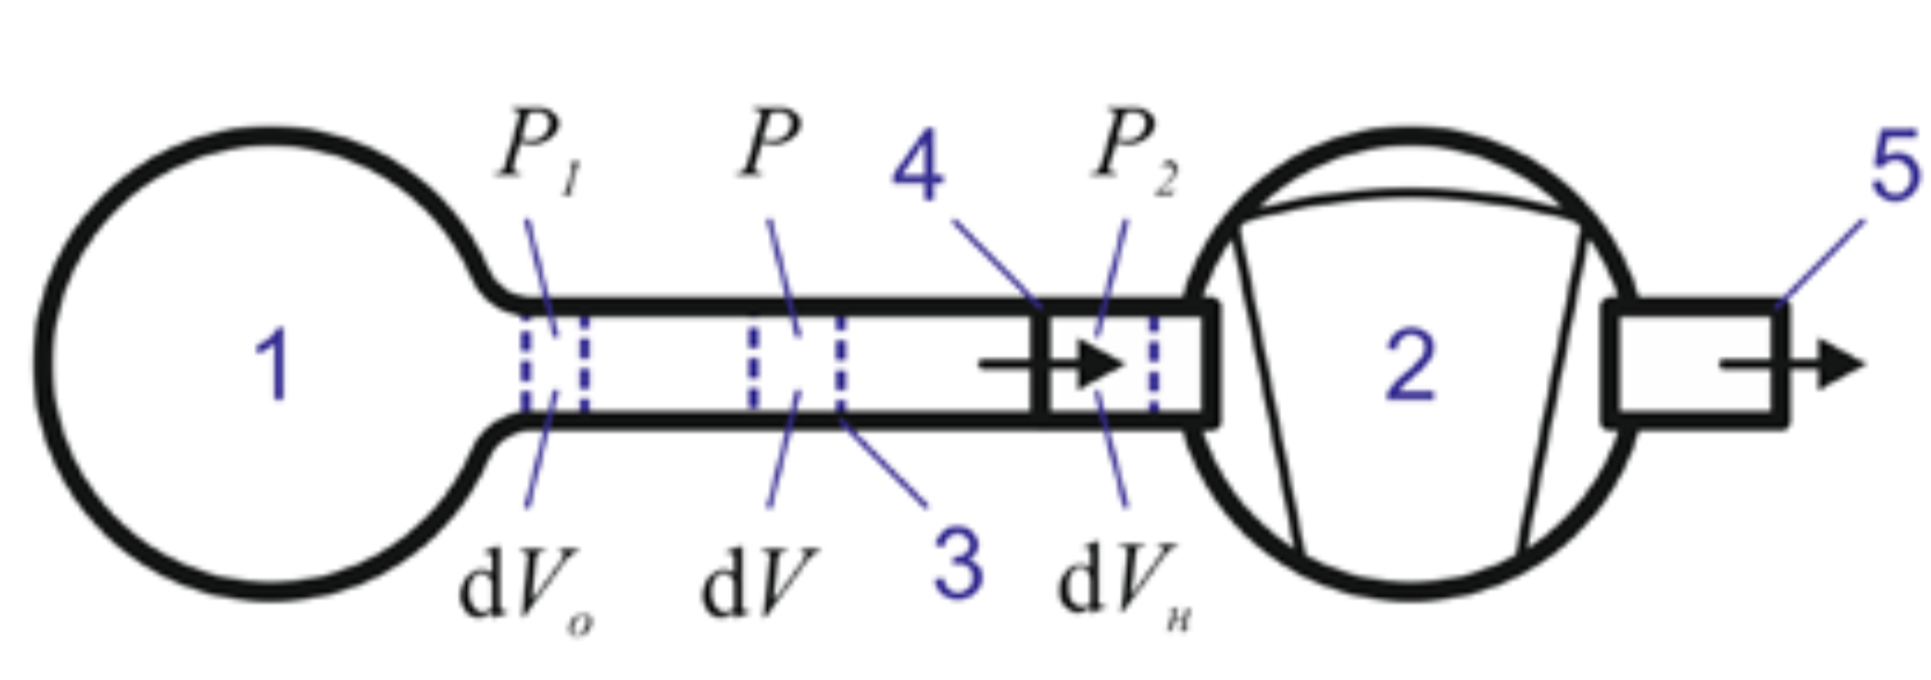
\includegraphics[width=\linewidth]{1}
    \captionsetup{justification=centering}
    \caption{Петля гистерезиса
    ферромагнетика}
\end{wrapfigure}

Индукция $\vec B$ в образце состоит из
индукции, связанной с намагничивающим
полем $\vec H$, и индукции, создаваемой самим
намагниченным образцом. В системе СИ эта
связь имеет вид
\begin{equation}
    \vec B = \mu_0(\vec H + \vec M),
\end{equation}
где $\vec M$ -- намагниченность --
магнитный момент единичного объёма
образца, а $\mu_0$ — магнитная постоянная.
Кривая $OACD$, изображающая зависимость
$B(H)$, практически совпадает с
зависимостью $M(H)$, поскольку второй
член в выражении (1) — в малых
полях — существенно превосходит
первый. В точке $C$ 
намагниченность $M$ достигает
насыщения, и дальнейшее
медленное увеличение индукции
происходит в основном вследствие
роста $H$.

Намагнитим образец до насыщения — до
точки $D$. Соответствующее значение
индукции $B_s$ называют индукцией
насыщения. При уменьшении поля $H$ до нуля
зависимость $B(H)$ имеет вид кривой $DCE$, и
при нулевом поле индукция имеет конечное
— ненулевое — значение. Это остаточная
индукция $B_r$. Чтобы размагнитить образец,
то есть перевести его в состояние $F$,
необходимо приложить <<обратное>>
магнитное поле $H_c$, которое называют
коэрцитивной силой.

Замкнутая кривая $DEFD'E'F'D$, возникающая
при циклическом перемагничивании
образца, намагниченного до насыщения,
называется предельной петлёй
гистерезиса.

В работе исследуются ферромагнитные
образцы тороидальной формы.

\begin{figure}[H]
    \centering
    \begin{floatrow}
        \ffigbox{
            \captionsetup{justification=centering}
            \caption{Схема для измерения
            индукционного тока (или
        заряда)}
        }
        {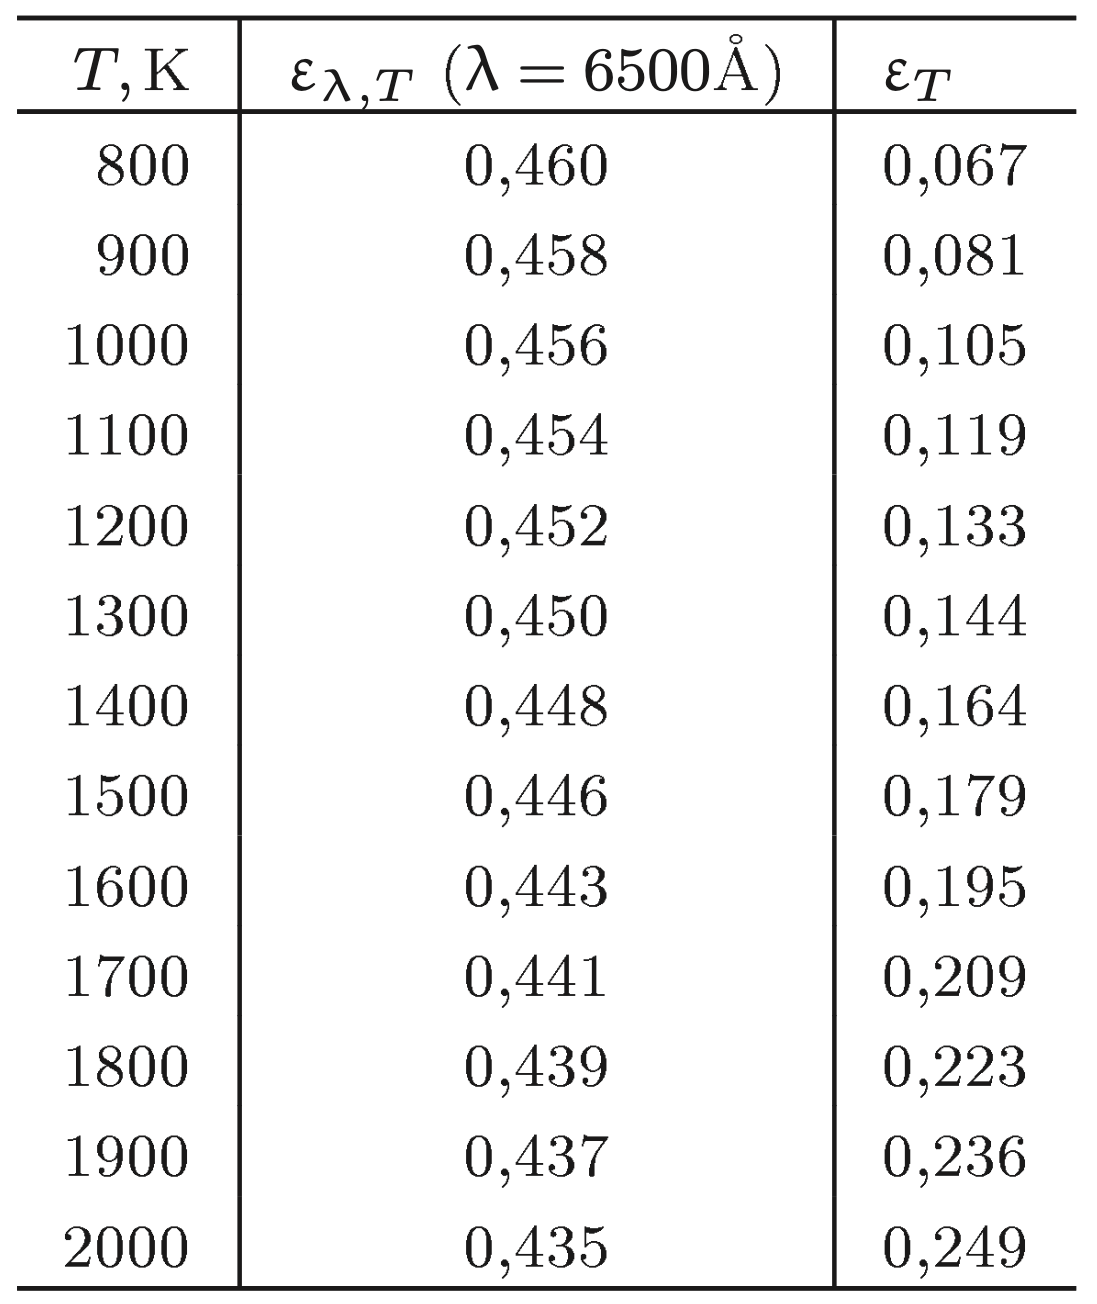
\includegraphics[width=0.9\linewidth]{2}}
        \ffigbox{
            \captionsetup{justification=centering}
            \caption{Схема для
            калибровки гальванометра}
        }
        {
            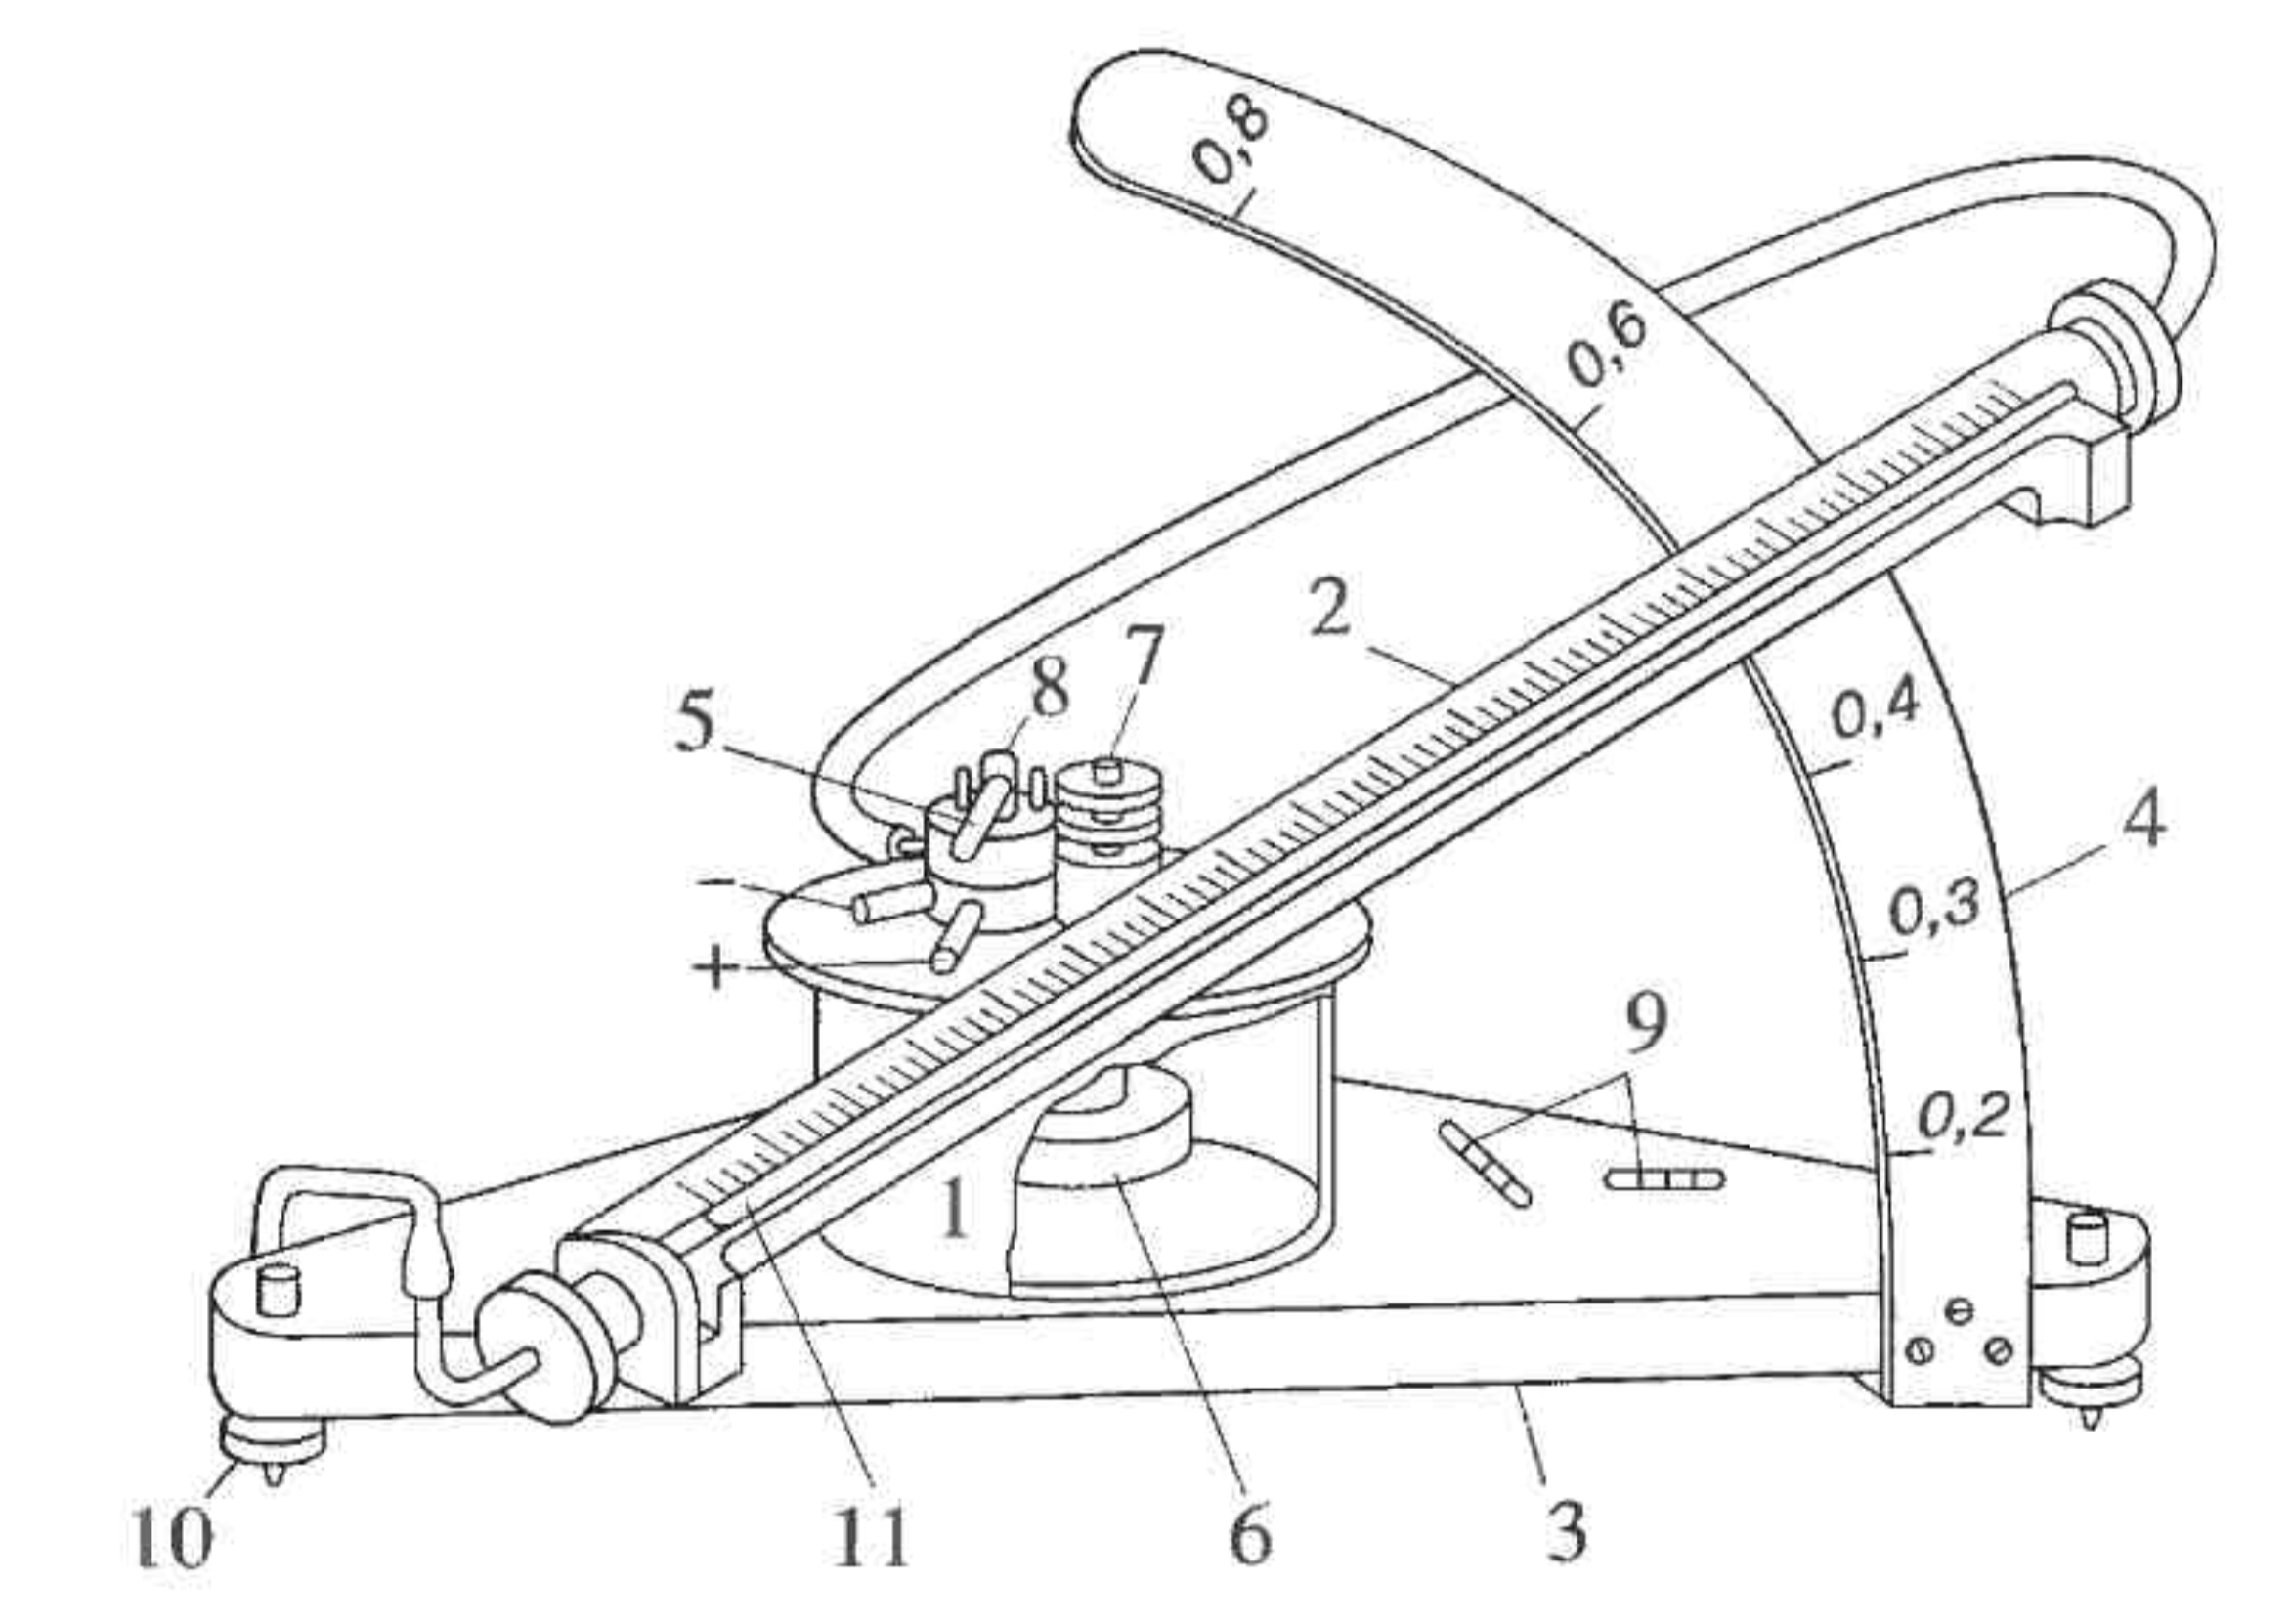
\includegraphics[width=0.6\linewidth]{3}
        }
        
    \end{floatrow}
\end{figure}
Изложим суть метода. На
тороидальный сердечник (рис. 2)
равномерно намотана намагничивающая
обмотка с числом витков $N_{T0}$, а поверх
неё — измерительная обмотка с числом
витков $N_{T1}$.

Если быстро изменить ток в
намагничивающей обмотке, то в
измерительной обмотке возникает ЭДС
индукции. Ток, вызванный этой ЭДС, течёт
через гальванометр Г, который работает в
баллистическом (импульсном) режиме, то
есть реагирует на полный заряд,
протекший через катушку гальванометра.

Напряжённость поля $H$ в сердечнике
пропорциональна току $I$ в первичной
обмотке $N_{T0}$, а изменение магнитной
индукции $B$ — заряду, протекшему через
гальванометр при изменении тока
намагничивания. Таким образом, измеряя
токи, текущие через обмотку $N_{T0}$, и
суммируя отклонения гальванометра,
подключённого к обмотке $N_{T1}$, можно
рассчитать зависимость $B(H)$ для
материала сердечника.

Рассмотрим подробнее, как выразить $B$
и $H$ 
через параметры, измеряемые в
эксперименте. Напряжённость магнитного
поля $H$ в тороиде зависит от тока,
текущего в намагничивающей обмотке:
\begin{equation}
    H = \frac{N_{T0}}{\pi D}I,
\end{equation}
где $D$ -- средний диаметр тора.

Пусть в намагничивающей обмотке ток
скачкообразно изменился на величину
$\Delta I$.
При этом меняется поле $H$ в тороиде:
$\Delta H \sim \Delta I$.

Изменение поля $\Delta H$ приводит к изменению
потока магнитной индукции $\Phi$ в
сердечнике, и в измерительной обмотке
сечения $S_T$ с числом витков $N_{T1}$ возникает
ЭДС индукции:
\[
    \mathscr{E} = - \frac{d\Phi}{dt} =
    -S_T N_{T1} \frac{dB}{dt}
\]

Через гальванометр Г протекает импульс
тока; первый отброс зайчика
гальванометра, работающего в
баллистическом режиме, пропорционален
величине прошедшего через гальванометр
заряда $q$:

\[
\varphi = \frac{q}{b}
\]
Коэффициент пропорциональности $b$ 
называют баллистической постоянной
гальванометра.

Свяжем отклонение зайчика $\varphi$ с
изменением магнитной индукции $\Delta
B$:

\begin{equation}
    |\varphi| = \frac{q}{b} =
    \frac{1}{b}\int I dt = \frac{1}{bR}
    \int \mathscr{E} dt = \frac{S_T
    N_{T1}}{bR}\Delta B
\end{equation}
где $R$ -- полное сопротивление
измерительной цепи тороида, $S_T$ --
площадь поперечного сечения сердечника:
$S_T = \pi d_T^2/4$.

Баллистическую постоянную $b$ можно
определить, если провести аналогичные
измерения, взяв вместо тороида с
сердечником пустотелый соленоид с числом
витков $N_{C0}$ на который намотана короткая
измерительная катушка с числом витков
$N_{C1}$ (рис. 3). В длинном соленоиде
(практически достаточно, чтобы его длина
превышала 6 диаметров: $l_c > 6d_c$)
поле $H$
можно рассчитать так же, как для тороида
(см. (2)); $B$ и $H$ в соленоиде связаны
линейно, поэтому связь между изменением
тока $\Delta I_1$ в обмотке $N_{C0}$ и изменением
магнитной индукции $\Delta B_C$ имеет простой
вид:

\begin{equation}
    \Delta B_C = \frac{\mu_0
    N_{C0}}{l_C}\Delta I_1
\end{equation}

Изменение магнитной индукции в соленоиде
связано с отклонением $\varphi_1$ зайчика
гальванометра формулой, аналогичной
формуле (3):
\begin{equation}
    \varphi_1 = \frac{S_C
    N_{C1}}{bR_1}\Delta B_C
\end{equation}
Здесь $R_1$ — полное сопротивление
измерительной цепи соленоида, $S_C$ —
площадь поперечного сечения соленоида:
$S_C = \pi d_C^2/4$.

Таким образом, выражения (3), (4) и (5)
позволяют, исключив баллистическую
постоянную $b$, установить связь между
отклонением зайчика в делениях $\Delta
x$ ($\Delta x \sim \varphi$) и
изменением магнитной индукции $\Delta x
\sim B$ в сердечнике тороида:

\begin{equation}
    \Delta B [T] = \mu_0 \left(
    \frac{d_C}{d_T} \right)^2
    \frac{R}{R_1}\frac{N_{C0}}{N_{T1}}\frac{N_{C1}}{l_C}\Delta
    I_1 \frac{\Delta x}{\Delta x_1}
\end{equation}

Строго говоря, величина $b$ — это не
константа. Она зависит не только от
параметров гальванометра, но и от
сопротивления цепи, к которой подключён
гальванометр, поэтому формула (6)
справедлива, если полные сопротивления
измерительных цепей тороида и соленоида
одинаковы: $R = R_1$.

\section{Оборудование}
\textbf{В работе используются:}
генератор тока с блоком питания, торо-
ид, соленоид, баллистический
гальванометр с осветителем и шкалой,
амперметры, магазин сопротивлений,
лабораторный автотрансформатор (ЛАТР),
разделительный трансформатор.d
\subsection*{Экспериментальная установка}
Схема для исследования петли гистерезиса
представлена на рис. 4. К блоку питания
(источнику постоянного напряжения)
подключён специальный генератор,
позволяющий скачками менять токи в
намагничивающей обмотке. Одинаковые
скачки $\Delta I (\sim \Delta H)$ вызовут разные
отклонения $\Delta x$ ($\sim \Delta B$)
на участках $FD'$ и $D'E'$: рис. 1
скачок $\Delta H_1$ может дать и $\Delta
B_1$ 
и $\Delta B_2$. Поэтому генератор меняет ток
неравномерно: большими скачками вблизи
насыщения и малыми вблизи нуля.

\begin{figure}[H]
    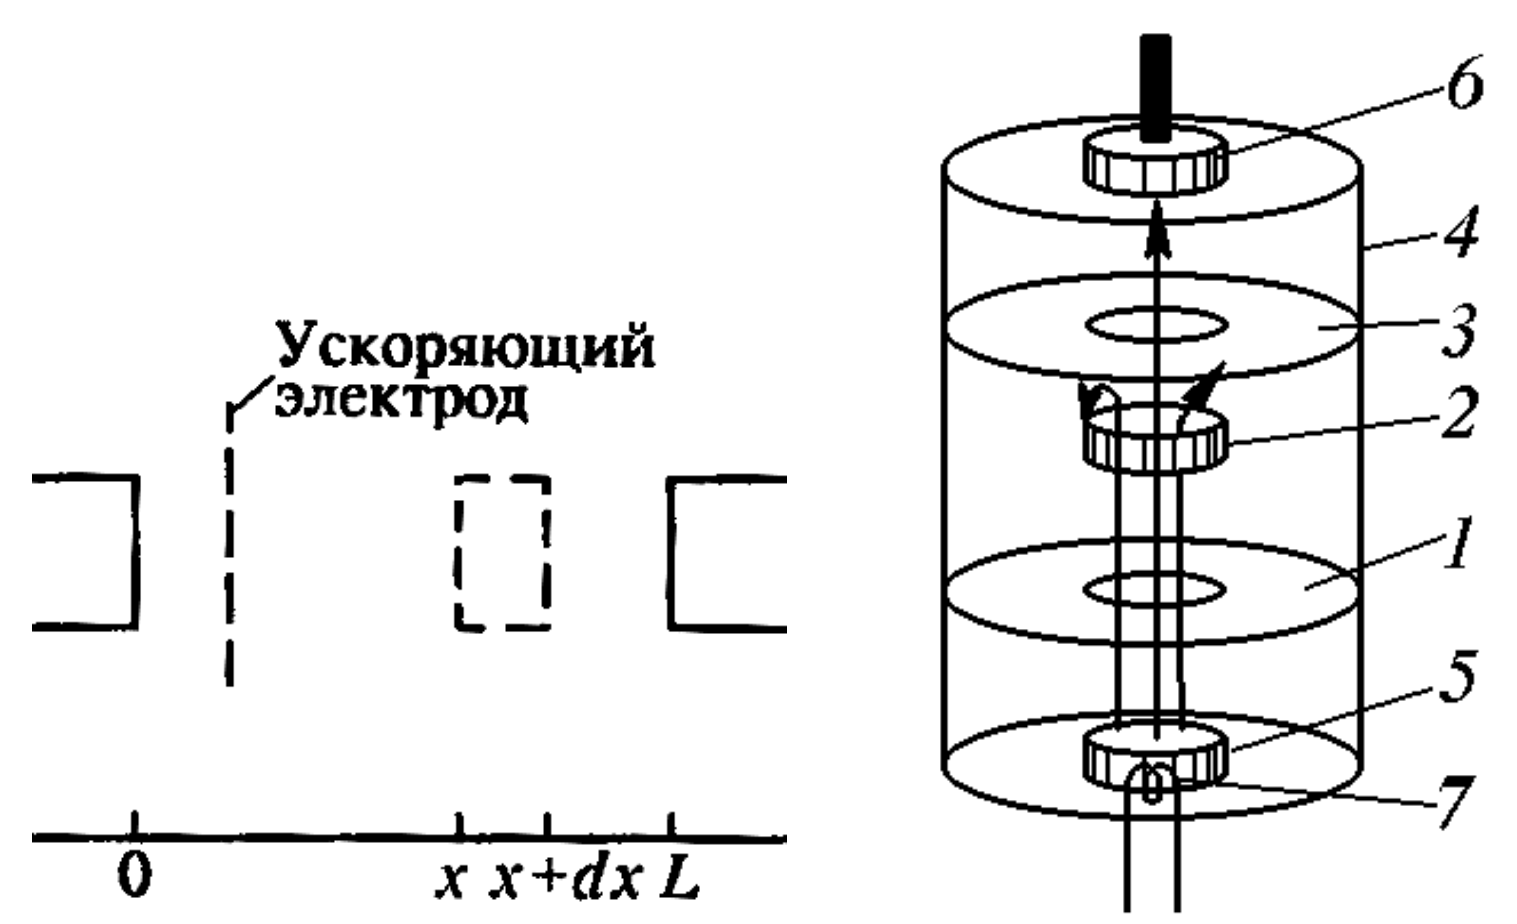
\includegraphics[width=\linewidth]{4} 
    \captionsetup{justification=centering}
    \caption{Схема установки для
    исследования петли гистерезиса}
\end{figure}

Ток в намагничивающей обмотке измеряется
амперметром $\text{A}_1$ с пределом 0,75 А при
малых токах или амперметром $\text{A}_2$ с
пределом 3 А в области насыщения. При
токах больше 0,75 А амперметр
$\text{A}_1$ должен
быть закорочен: ключ $\text{К}_1$ замкнут.
(Сопротивление амперметра мало и
сравнимо с сопротивлением ключа, поэтому
показания амперметра $\text{А}_1$ не падают до
нуля даже при замкнутом ключе.)
Переключатель $\text{П}_1$ позволяет менять
направление тока в первичной обмотке.

Чувствительность гальванометра Г во
вторичной цепи можно менять с помощью
магазина сопротивлений $R_M$· Ключ
$\text{К}_2$
предохраняет
гальванометр от перегрузок и замыкается
только на время измерения отклонений
зайчика. Ключ $\text{К}_0$ служит для мгновенной
остановки зайчика (короткое замыкание
гальванометра). Переключателем
$\text{П}_2$ можно
изменять направление тока через
гальванометр.

Схема на рис. 5 отличается от схемы на
рис. 4 только тем, что вместо тороида
подключён калибровочный соленоид.

Сопротивления измерительных цепей
тороида ($R = R_T + R_M + R_0$) и соленоида
($R_1 = R_C + R_M' + R_0$) должны быть
одинаковы [см. замечание после формулы
(6)].
\begin{figure}[H]
    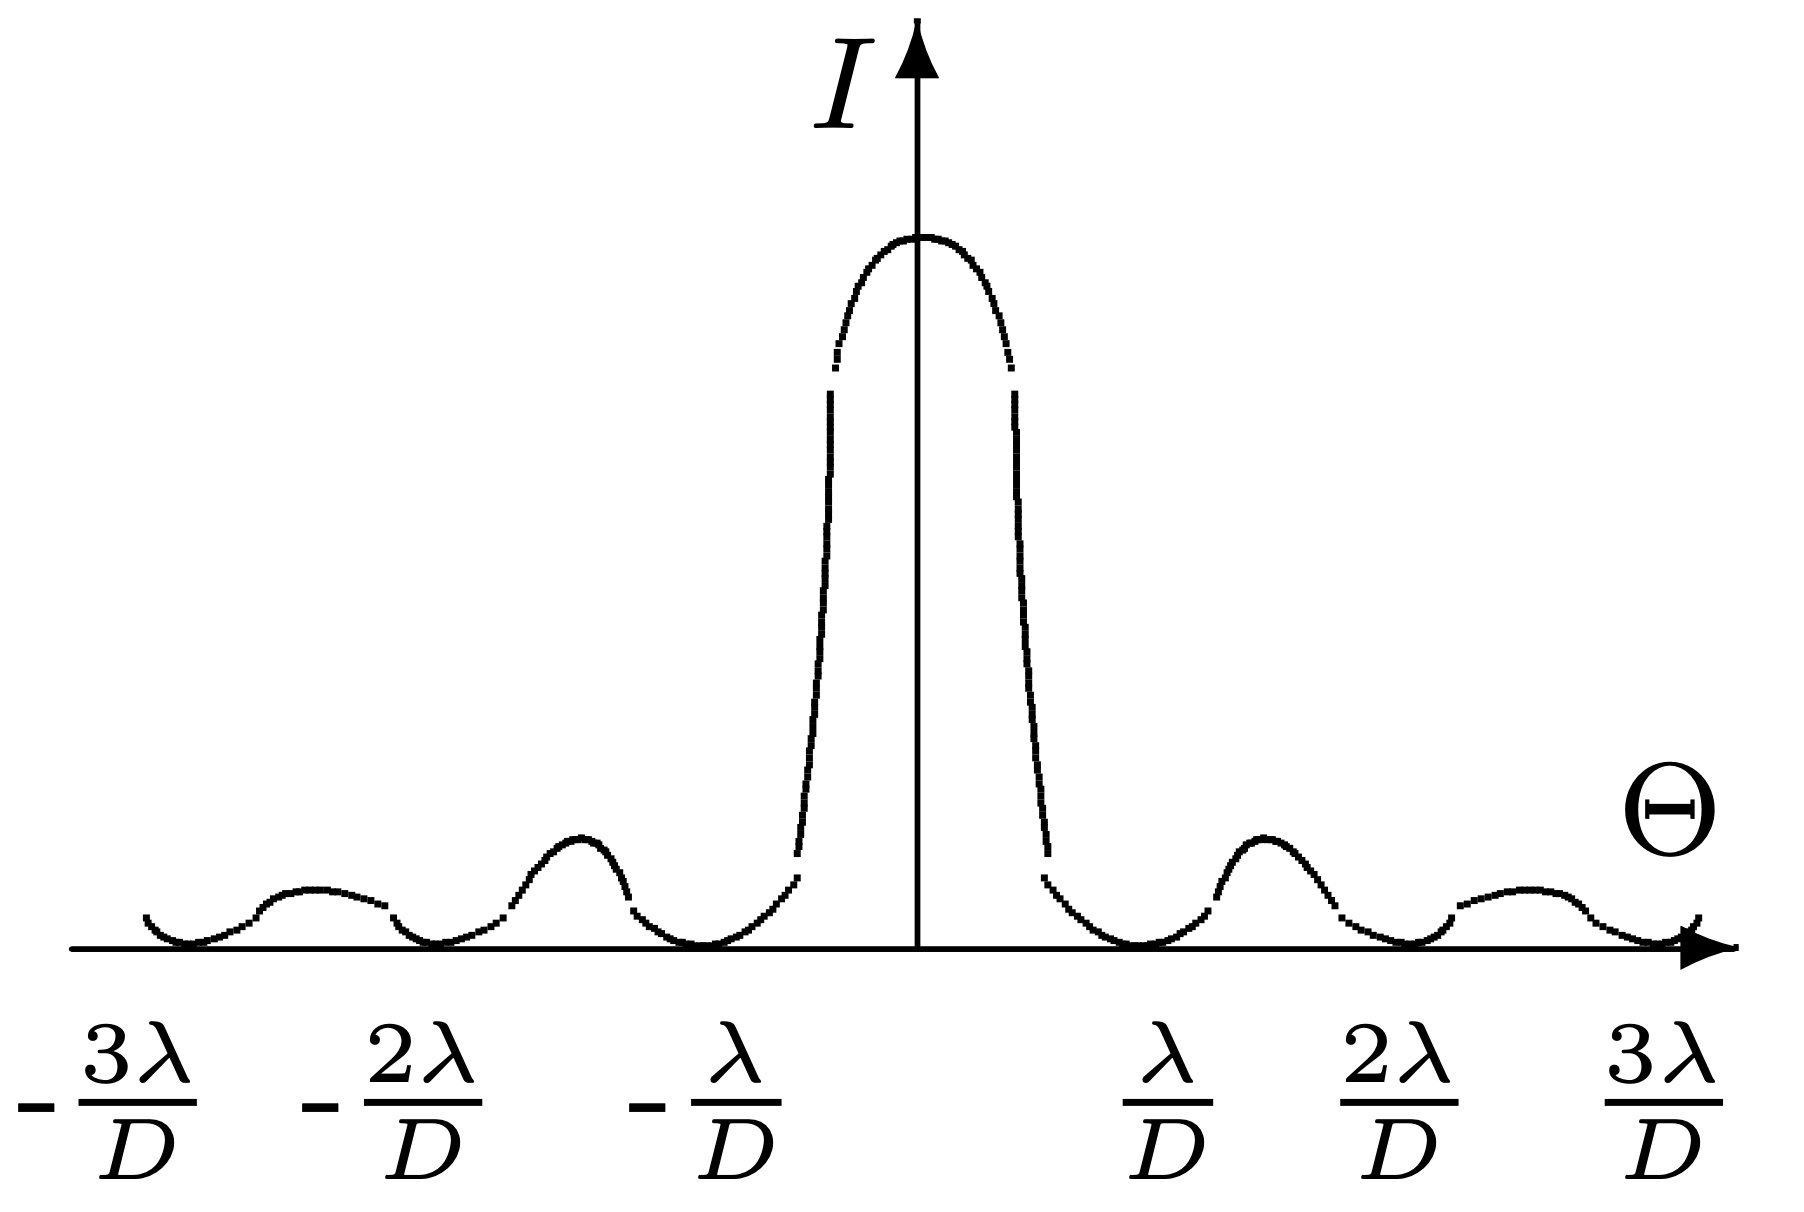
\includegraphics[width=\linewidth]{5} 
    \captionsetup{justification=centering}
    \caption{ Схема установки для
    калибровки гальванометра }
\end{figure}

\begin{wrapfigure}[8]{r}{0.35\linewidth}
    \vspace{-2ex}
    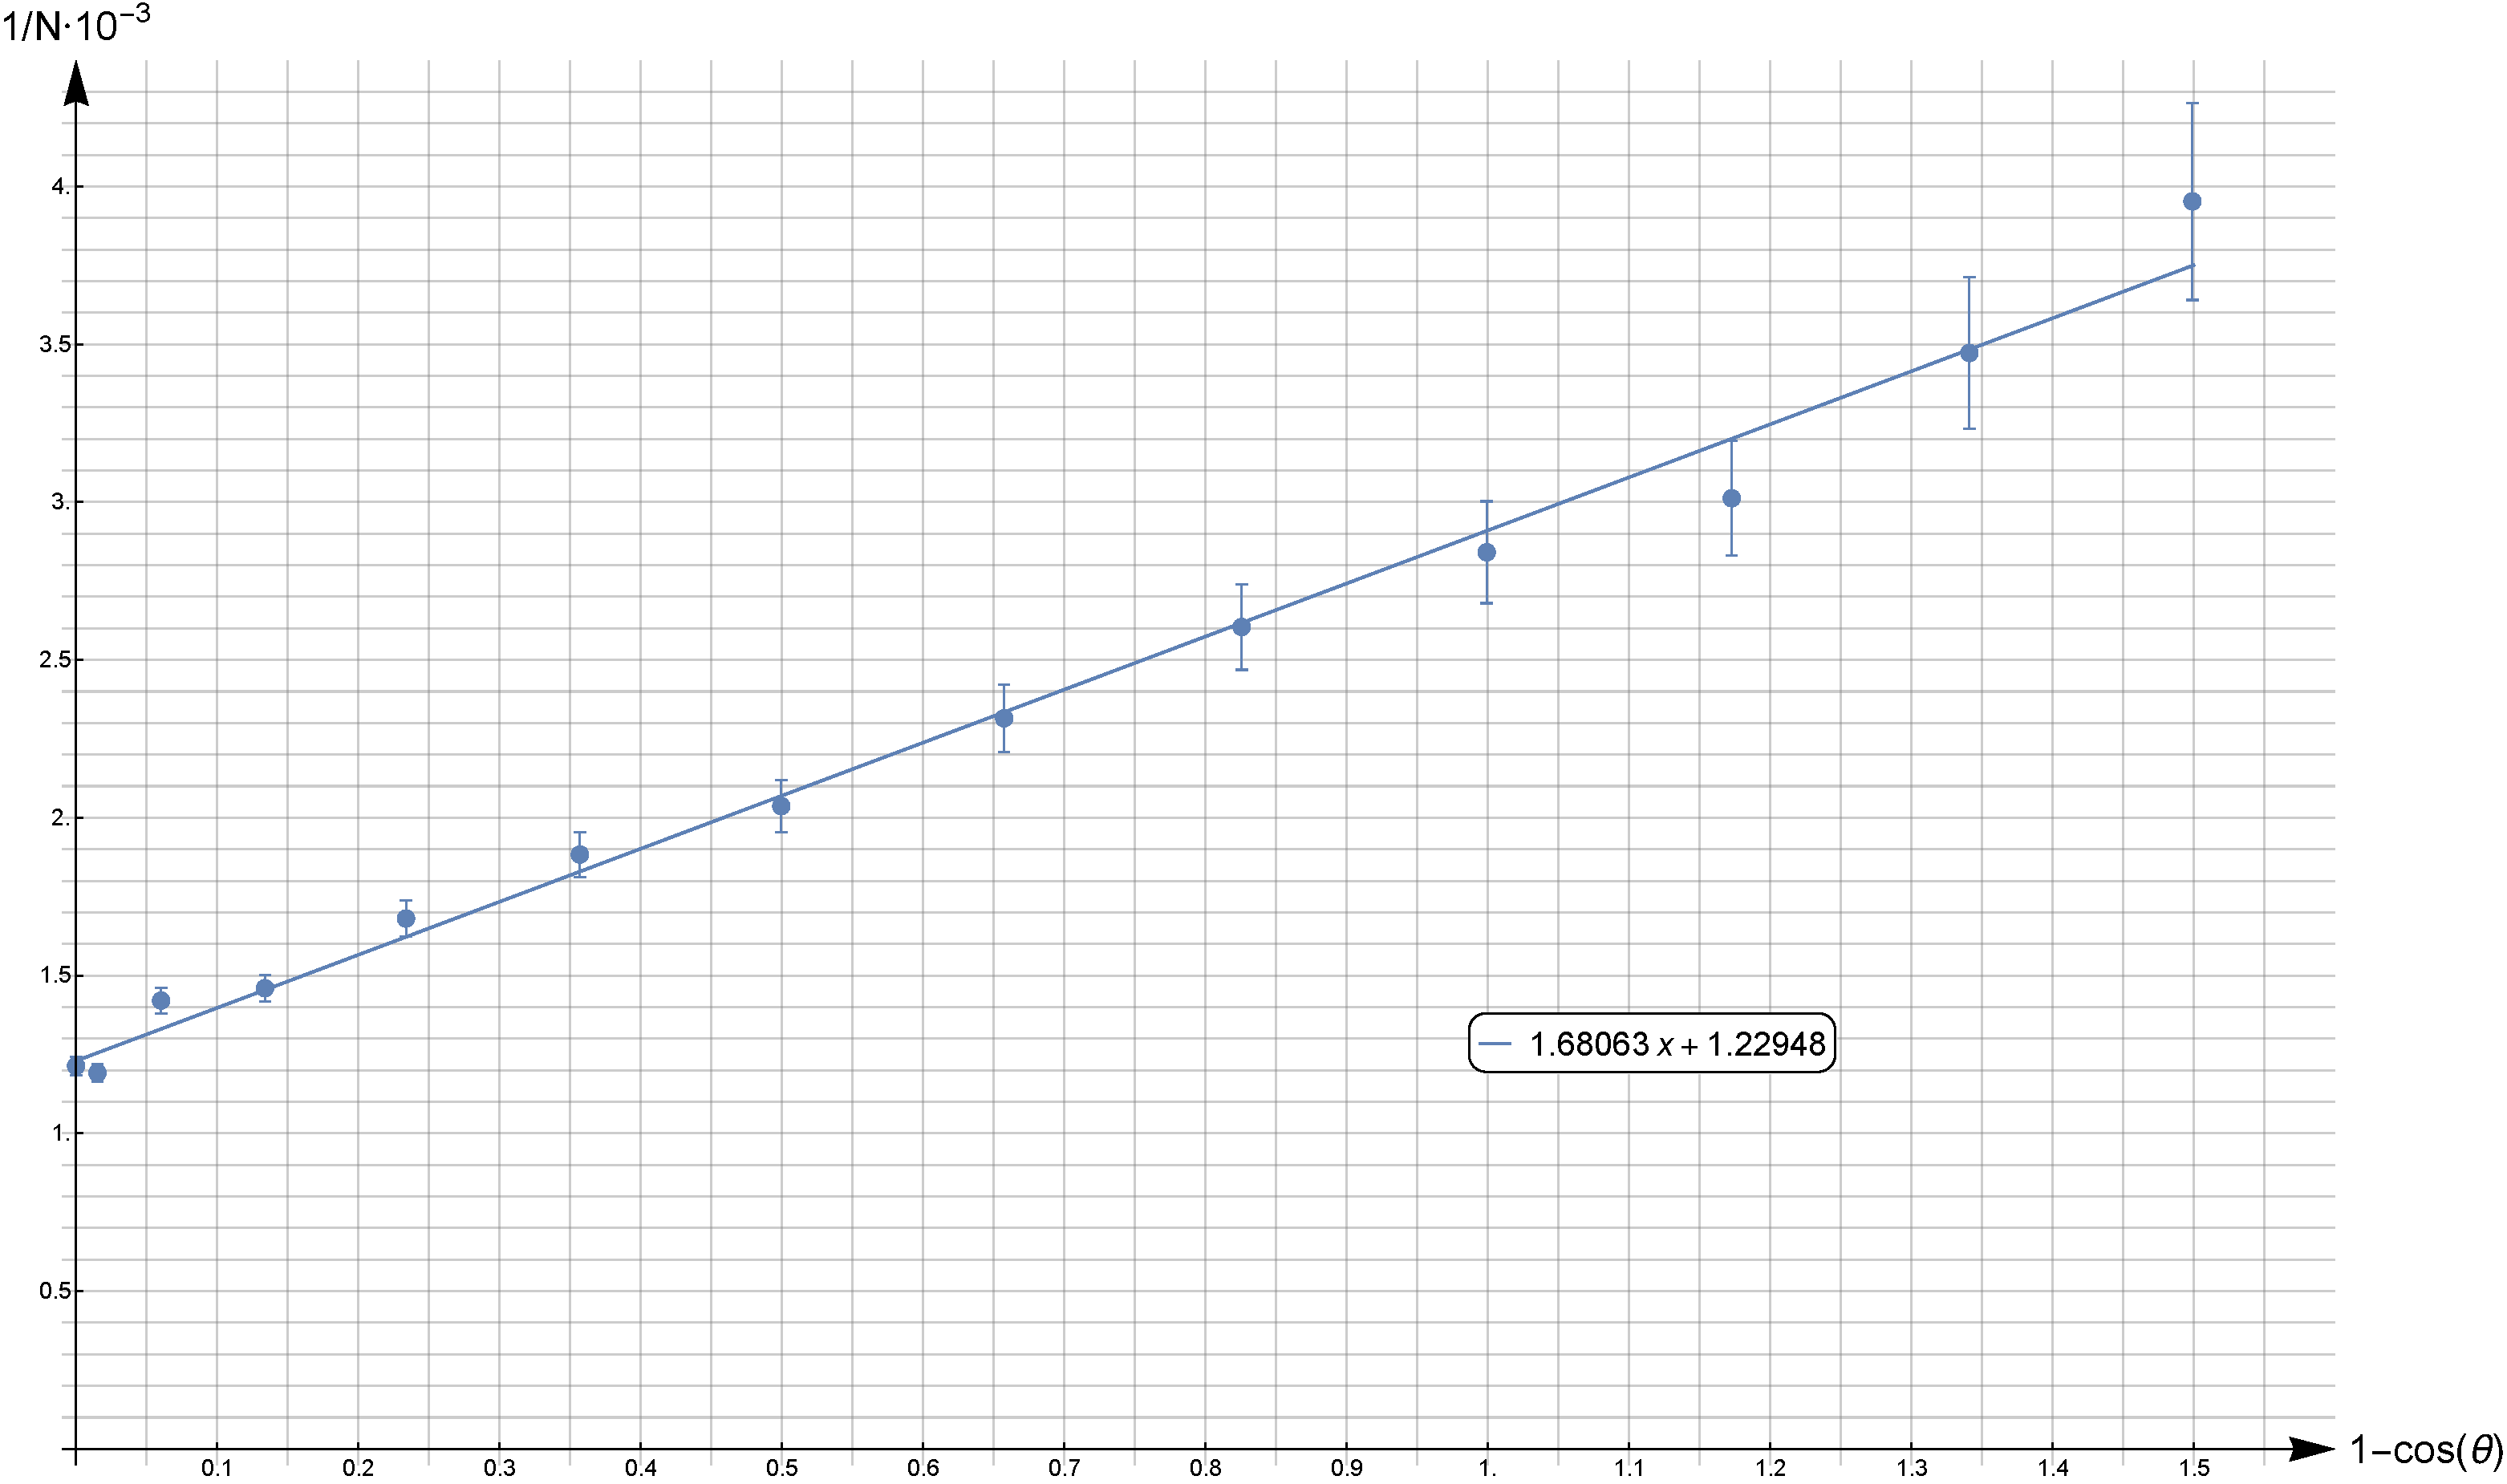
\includegraphics[width=\linewidth]{6}
    \captionsetup{justification=centering}
    \caption{Схема установки для
    размагничивания образца}
\end{wrapfigure}

Сопротивление тороида $R_T \ll R_0$ —
сопротивления гальванометра, поэтому
сопротивления магазина в схеме с
тороидом и соленоидом отличаются на
величину сопротивления соленоида $R_C:
R_M = R_C + R_M'$

Чтобы снять начальную кривую
намагничивания, нужно размагнитить
сердечник. Для этого тороид подключается
к цепи переменного тока (рис.~6). При
уменьшении амплитуды тока через
намагничивающую обмотку от тока
насыщения до нуля характеристики
сердечника $B$ и $H$ <<пробегают>>
за секунду 50 петель всё меньшей площади
и в итоге приходят в нулевую точку.



\section{Результаты измерений и обработка результатов}

Измерим предельной петлю гистерезиса.
Снимаем зависимость отклонения зайчика
$\Delta x$
от величины тока $I$.

\renewcommand{\arraystretch}{1} 
\begin{table}[H]
\centering
\begin{tabular}{|c|c|c|c|c|c|c|c|}
\hline
\multicolumn{2}{|c|}{$E'F'CD$} &
\multicolumn{2}{c|}{$DCE$} &
\multicolumn{2}{c|}{$EFC'D'$} &
\multicolumn{2}{c|}{$D'C'E'$} \\ \hline
$I, \ \text{мА}$            &
$\Delta x, \text {мм}$           &$I, \
\text{мА}$ 
             & $\Delta x, \
\text{мА}$          &$I, \ \text{мА}$ 
             & $\Delta x, \
\text{мм}$          &$I, \ \text{мА}$ 
             & $x, \ \text{мм}$           \\ \hline
0    &  --   & 1460 & 134  & 0     & -26  & -1460  & -136 \\ \hline
15   & 54  & 510  & -138 & -15   & -51  & -510   & 136  \\ \hline
28   & 63  & 251  & -118 & -28   & -69  & -250   & 128  \\ \hline
39   & 116 & 157  & -80  & -39   & -166 & -157   & 79   \\ \hline
45   & 116 & 95   & -66  & -45   & -116 & -95    & 74   \\ \hline
56   & 179 & 67   & -43  & -56   & -186 & -67    & 24   \\ \hline
67   & 95  & 56   & -16  & -67   & -96  & -56    & 9    \\ \hline
95   & 162 & 45   & -17  & -95   & -172 & -45    & 7    \\ \hline
157  & 166 & 39   & -7   & -157  & -176 & -39    & 4    \\ \hline
251  & 119 & 28   & -10  & -251  & -120 & -28    & 7    \\ \hline
500  & 146 & 15   & -13  & -520  & -154 & -15    & 8    \\ \hline
1460 & 134 & 0    & -26  & -1460 & -136
     & 0      & 26  \\  \hline
\end{tabular}
\captionsetup{justification=centering}
\caption{
Зависимость отклонения зайчика
$\Delta x$
от величины тока $I$.
}
\end{table}

Используя формулы (2) и (6) получим
зависимость магнитной индукции $B$ от
напряженности магнитного поля $H$.
\renewcommand{\arraystretch}{1.05} 
\begin{table}[H]
\centering
\begin{tabular}{|c|c|c|c|c|c|c|c|}
\hline
\multicolumn{2}{|c|}{$E'F'CD$} &
\multicolumn{2}{c|}{$DCE$} &
\multicolumn{2}{c|}{$EFC'D'$}   &
\multicolumn{2}{c|}{$D'C'E'$} \\ \hline
 $H, \
\text{А/м}$        & $B, \ \text
{мТл}$  &   $H, \
\text{А/м}$
& $B, \ \text
{мТл}$            & $H, \
\text{А/м}$
& $B, \ \text
{мТл}$         & $H, \
\text{А/м}$
& $B, \ \text
{мТл}$        \\ \hline
0,00    & -512,21 & 8132,80 & 1247,30 & 0,00     & 551,31   & -8132,80 & -1328,11 \\ \hline
85,78   & -441,83 & 2840,91 & 1067,44 & -85,78   & 484,84   & -2840,91 & -1150,85 \\ \hline
156,53  & -359,72 & 1398,17 & 913,64  & -156,64  & 394,91   & -1392,60 & -984,03  \\ \hline
218,14  & -208,54 & 874,55  & 809,38  & -218,14  & 178,56   & -874,55  & -881,06  \\ \hline
247,88  & -57,35  & 529,19  & 723,36  & -247,88  & 27,37    & -529,19  & -784,61  \\ \hline
311,94  & 175,95  & 371,55  & 667,31  & -311,94  & -215,05  & -371,55  & -753,33  \\ \hline
371,55  & 299,77  & 311,94  & 646,46  & -371,55  & -340,17  & -311,94  & -741,60  \\ \hline
528,63  & 510,91  & 247,88  & 624,30  & -528,07  & -564,35  & -247,88  & -732,48  \\ \hline
876,23  & 727,27  & 218,36  & 615,18  & -876,78  & -793,74  & -218,36  & -727,27  \\ \hline
1395,94 & 882,36  & 156,53  & 602,15  & -1396,50 & -950,14  & -156,53  & -718,14  \\ \hline
2785,20 & 1072,65 & 85,78   & 585,20  & -2896,61 & -1150,85 & -85,78   & -707,72  \\ \hline
8132,80 & 1247,30 & 0,00    & 551,31  & -8132,80 & -1328,11 & 0,00     & -673,83  \\ \hline\end{tabular}
\captionsetup{justification=centering}
\caption{Зависимость магнитной индукции
$B$ от напряженности магнитного поля $H$}
\end{table}

Построим петлю гистерезиса $B = f(H)$ с
начальной кривой намагничивания.

\begin{table}[H]
\centering
\begin{tabular}{|c|c|c|c|}
\hline
$I, \ \text{мА}$    & $dx, \ \text{мм}$
& $H, \ \text{А/м}$       & $B, \
\text{мТл}$       \\ \hline
0    &  --   & 0       & 0       \\ \hline
15   & 20  & 85,78   & 26,07   \\ \hline
28   & 34  & 156,53  & 70,38   \\ \hline
39   & 68  & 218,08  & 159,01  \\ \hline
45   & 38  & 247,88  & 208,54  \\ \hline
56   & 78  & 311,94  & 310,20  \\ \hline
67   & 58  & 371,55  & 385,79  \\ \hline
95   & 120 & 529,19  & 542,19  \\ \hline
157  & 120 & 874,55  & 698,59  \\ \hline
251  & 123 & 1398,17 & 858,90  \\ \hline
514  & 155 & 2863,19 & 1060,92 \\ \hline
1457 & 142 & 8116,09 & 1246,00 \\ \hline
\end{tabular}
\captionsetup{justification=centering}
\caption{Начальная кривая намагничивания}
\end{table}

\begin{figure}[H]
    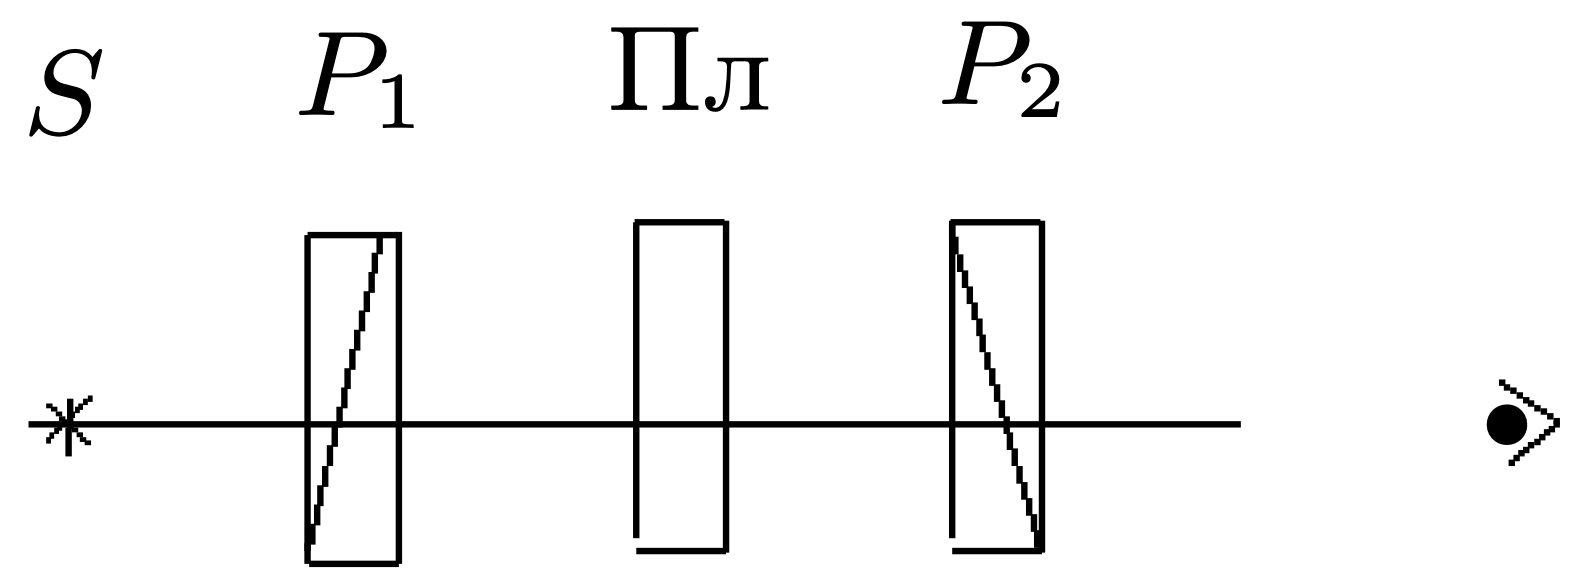
\includegraphics[width=\linewidth]{7} 
    \captionsetup{justification=centering}
    \caption{Петля гистерезиса $B = f(H)$ с
    начальной кривой намагничивания}
\end{figure}

Определим по графику коэрцитивную силу
$H_c$ и индукцию насыщения $B_s$
 \begin{equation*}
    \begin{aligned}
        H_c &= 270 \pm 40 \ \text{А/м}\\
        B_s &= 1,3 \pm 0,2 \ \text{Тл}
    \end{aligned}
\end{equation*}


Определим максимальное значение
дифференциальной магнитной проницаемости
$\mu_\text{дифф}$ для начальной кривой
намагничивания:
\[
    \mu_{\text{дифф}} =
    \frac{1}{\mu_0}\frac{dB}{dH}
\]
\[
    \mu_\text{дифф}^{\text{макс}} = 1280 \pm
    120
\]

\section{Обсуждение результатов и выводы}
Результаты занесены в таблицу.
\begin{table}[H]
    \begin{tabular}{|c|c|c|}
        \hline
        & Эксперим. & Справочн. \\
        \hline
        $H_c, \ \text{А/м}$ & $270 \pm
        40$
        & 80 \\ \hline
        $B_s, \ \text{Тл}$ & $1,3 \pm
        0,2$
        & 2,15 \\ \hline
        $\mu_\text{диф}$ & $1280 \pm 120$ &
        5000 \\  \hline
   \end{tabular}
    \captionsetup{justification=centering}
    \caption{Результаты измерений
    коэрцитивной силы $H_c$, индукции
насыщения $B_s$ и дифференциальной
магнитной проницаемости
$\mu_\text{дифф}$ для начальной кривой
намагничивания }
\end{table}


\end{document}

